\documentclass{article}
\usepackage{amsmath,amsthm,amssymb,amsfonts}
\usepackage{setspace,enumitem}
\usepackage{graphicx}
\usepackage{hyperref}
\usepackage{natbib}
\usepackage{afterpage}
\usepackage{xcolor}
\usepackage{etoolbox}
\usepackage{booktabs}
\usepackage{pdfpages}
\usepackage{multicol}
\usepackage{geometry}
\usepackage{accents}
\usepackage{bbm}
\usepackage{placeins}
\hypersetup{
	colorlinks,
	linkcolor={blue!90!black},
	citecolor={red!90!black},
	urlcolor={blue!90!black}
}

\newtheorem{theorem}{Theorem}
\newtheorem{assumption}{Assumption}
\newtheorem{definition}{Definition}
\newtheorem{lemma}{Lemma}
\setlength{\parindent}{0cm}
\geometry{margin = 1in}

\newcommand{\R}{\mathbb{R}}
\newcommand{\ubar}[1]{\underaccent{\bar}{#1}}
\newcommand{\Int}{\text{Int}}
\newcommand{\xbf}{\mathbf{x}}
\newcommand{\Abf}{\mathbf{A}}
\newcommand{\Bbf}{\mathbf{B}}
\newcommand{\Gbf}{\mathbf{G}}
\newcommand{\bbf}{\mathbf{b}}
\newcommand{\one}{\mathbbm{1}}

\newtoggle{extended}
\settoggle{extended}{false}

\title{ECON 810: Homework 5}
\author{Alex von Hafften }

\begin{document}

\maketitle

See assignment for model description.

\begin{enumerate}

\item Show if the child's human capital function exhibits dynamic complementarity.  How do you think this will impact your results?

Consider the human capital law of motion for children:

\begin{align*}
h^{c}_1 
&= (1 - \omega_c) h^c_0 + \gamma \omega_c i_1\\
h^{c}_2 
&= (1 - \omega_c) h^c_1 + \gamma \omega_c i_2\\
&= (1 - \omega_c)^2 h^c_0 + (1 - \omega_c) \gamma \omega_c i_1 + \gamma \omega_c i_2 \\
\frac{\partial h^{c}_2}{\partial i_2} &= \gamma \omega_c
\end{align*}

$\frac{\partial h^{c}_2}{\partial i_2}$ is a constant function with respect to $i_1$, so the human capital function does not exhibit dynamic complementarity.  This means that parents will not invest early in their children's human capital. My modified law of motion for child's human capital (see description below) also doesn't exhibit dynamic complementarity:

\begin{align*}
\exp(h^{c}_1)
&= (1 - \omega_c) \exp(h^c_0) + \gamma \omega_c i_1\\
\exp(h^{c}_2 )
&= (1 - \omega_c) \exp(h^c_1) + \gamma \omega_c i_2\\
&= (1 - \omega_c)^2 \exp(h^c_0) + (1 - \omega_c) \gamma \omega_c i_1 + \gamma \omega_c i_2 \\
\frac{\partial \exp(h^{c}_2)}{\partial i_2} &= \gamma \omega_c
\end{align*}

\item Solve and simulate data from the model using the suggested parameters above.

The attached code solves the model and simulates data:

\begin{itemize}

\item See \texttt{age\_profile.R} for the estimation of the age profile from PSID data.

\item See \texttt{model.jl} for code to estimate the model.

\item See \texttt{test.jl} for a test file.

\item See \texttt{simulation.jl} for code to simulate data from the model.

\item See \texttt{run.jl} for code to run the analysis of the model.

\end{itemize}

A few details on my approach in the problem set:

\begin{itemize}

\item I used CRRA utility with coefficient of constant risk aversion equal to two.

\item In the law of motion of child's human capital, I replaced $\kappa$ with $\gamma$ to avoid confusion with the age profile of earnings.

\item I used Tauchen for defining the human capital grid.

\item I changed the law of motion of child's human capital to 

$$
\exp(h^{c'}) = (1 - \omega_c) \exp(h^c) + \gamma \omega_c i
$$

I did this because as written in the problem set, human capital is subject to normal shocks, so it could be negative.  I was getting slightly counterintuitive results with $h^c$ was negative and the parents could investment nothing $(i = 0)$ and the human capital of the child would increase (i.e. to a less negative number). I think this approach is equivalent to using log normal shocks for human capital i.e. $\tilde{h} = \exp(h)$.

\item I increased $\gamma$ from 1/10 to 1/750 because, in my simulations, parents could invest very little and max out their child's human capital.  $\gamma = 1/750$ resulted in an interior distribution for $h$ at $t=4$.  This change makes human capital relatively more expensive.

\item When parents make investment choices for their child's human capital (i.e. $t=5, 6, 7, 8$), I do a grid search for each level of assets and level of child's human capital tomorrow.  I think back out the investment that is required for that level of child's human capital.  I don't allow negative investment nor negative consumption.  This approach keeps the child's human capital on the human capital grid.

\item A note on how I approached the simulations. I start all simulations at the lowest human capital level and zero assets.  I simulate each agent's life by applying policy function, human capital shocks, and drawing the child's initial human capital from a uniform distribution over the lower half of the human capital grid points.  Then I re-simulate by starting each simulation at the human capital level of the child when they live and the starting assets to the transfer the initial simulate round gave to their kids. I then repeat for 200 times.  In effect, I simulate 200 generations. I found that initial conditions (i.e. the first generation starts with high or low assets or human capital) does not qualitative change the simulation results after 200 generations.  I also tried something similar but simulating until convergence of the sup norm applied to the starting assets and human capital level, but with the error inherent in a monte carlo simulation prevented convergence. I thought simulating for a deterministic number of generations was better.

\end{itemize}

\item Plot policy functions for investment in the child's human capital.

\begin{itemize}

\item As expected from problem 1, parents do not invest in their child's human capital in $t=5, 6, 7$ because the human capital law of motion does not exhibit dynamic complementarity.  How I solved the model (i.e. by grid search over the level of child's human capital tomorrow, then backing out investment) leads parents to make small investments (between \$1 and \$50), but this is an artifact of the solution method.

\item Below I plot the investment in child's human capital in $t=8$.  I plot for policy function for a parent with the lowest level of human capital for all levels of the child's human capital, a parent with the highest level of human capital for all levels of child's human capital, a child with the lowest level of human capital for all levels of parent's human capital, and a child with the highest level of human capital for all levels of parent's human capital.  I highlight the lowest level of human capital in blue and the highest level in red.

\begin{center}

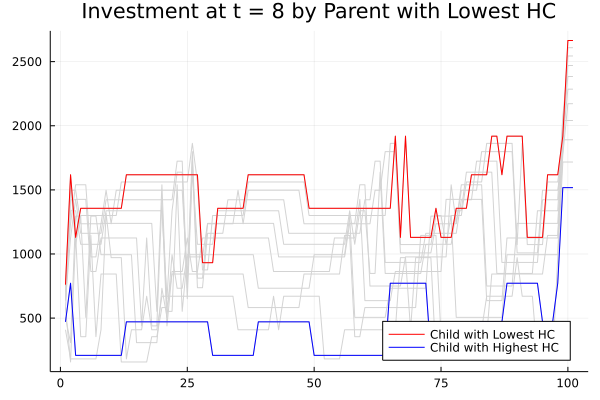
\includegraphics[scale =0.5]{i_p_l}

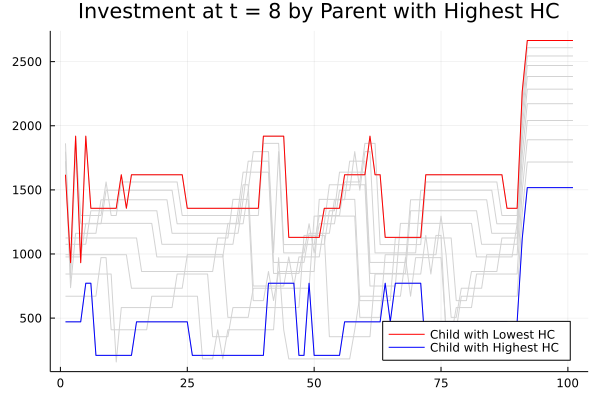
\includegraphics[scale =0.5]{i_p_h}

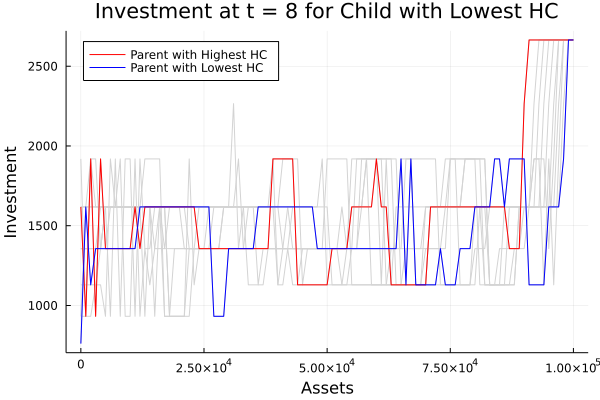
\includegraphics[scale =0.5]{i_c_l}

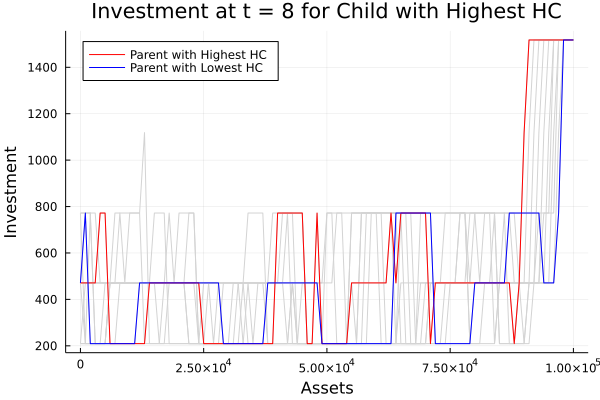
\includegraphics[scale =0.5]{i_c_h}

\end{center}

\item We see that children with the lower levels of human capital get a more investment than children with higher levels of human capital from the same parent.  But investments don't really look different across levels of parent's human capital.

\end{itemize}

\item Plot policy functions for the transfer that parents give to their children.

\begin{itemize}

\item I use a similar scheme for plotting transfer policy function:

\begin{center}

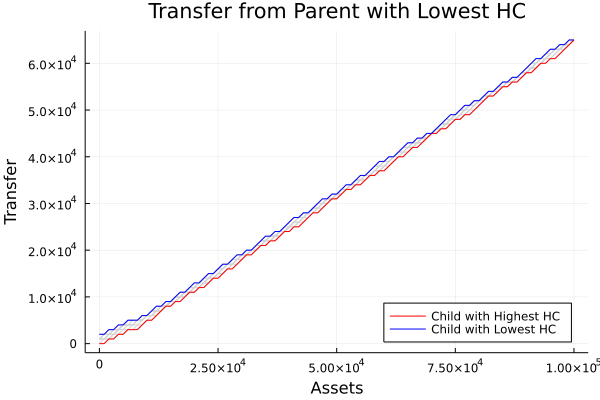
\includegraphics[scale =0.5]{tau_p_l}

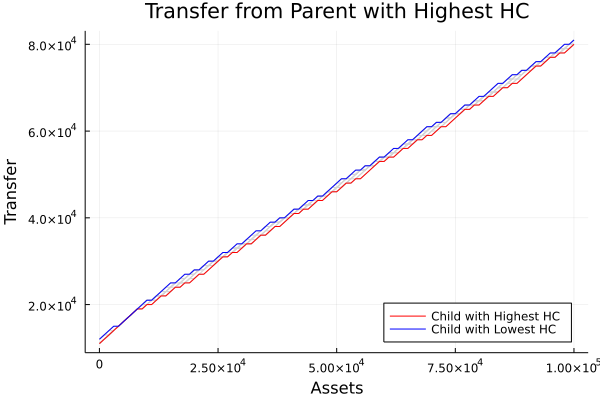
\includegraphics[scale =0.5]{tau_p_h}

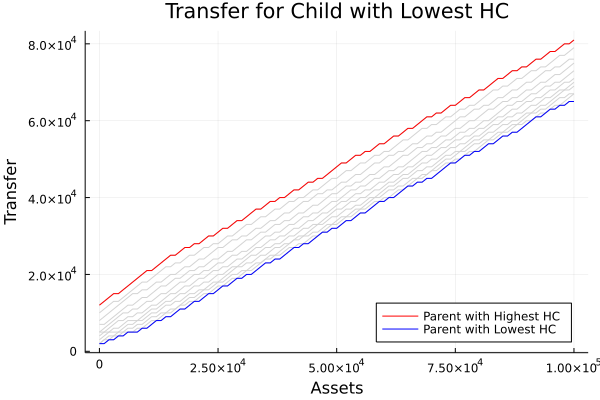
\includegraphics[scale =0.5]{tau_c_l}

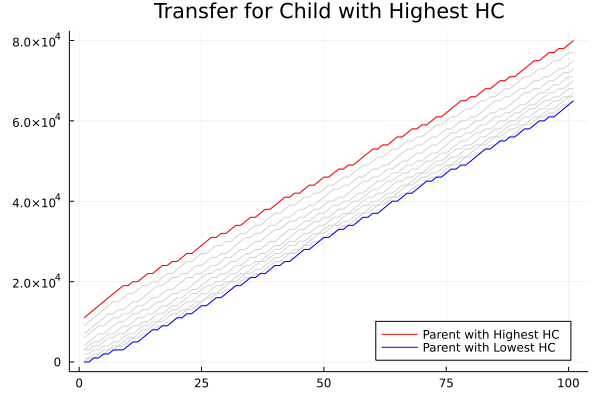
\includegraphics[scale =0.5]{tau_c_h}

\end{center}

\item Interestingly, we see the opposite result as human capital investment here.  We see that a parent will transfers about the same to their child regardless of their human capital (maybe slightly more for low human capital children).  But conditional on a child's human capital, a child will receive substantially more from a high human capital parent than a low human capital parent.  This is the income effect at work: a parent with high human capital has higher expected future earnings, so can transfer more to their child.  I wonder how this would change if the transfer occurred at the end of the parent's life (i.e. bequest).

\end{itemize}

\item Plot the distribution of human capital in the economy when agents enter the labor market.

I simulate the 10,000 agents. The histogram of human capital at $t=4$ is plotted below. 

\begin{center}

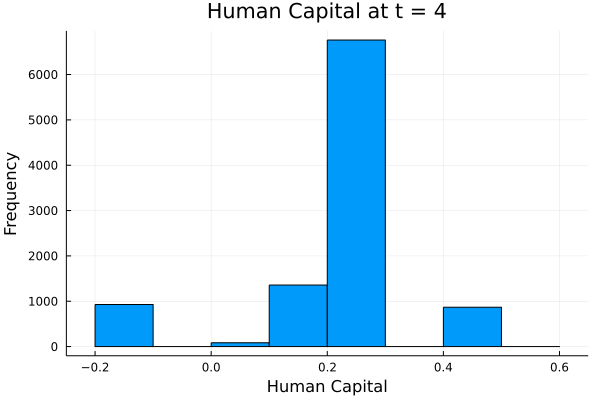
\includegraphics[scale =0.5]{hc_histogram}

\end{center}

As I mentioned above, I used different values of $\gamma$ and settled on $\gamma = 1/750$.  The max and min human capital grid point using Tauchen was $\pm 0.70484$, so you can see that this distribution is on the interior of the human capital points.  In general, it looks potentially Gaussian, with a large mass around the $0.25$.

\bigskip

The histogram of the transfers is plotted below:

\begin{center}

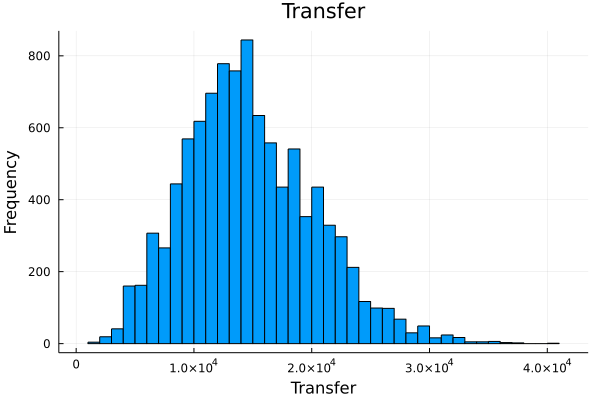
\includegraphics[scale =0.5]{transfer_histogram}

\end{center}

\item Plot the variance of earnings as a function of age in the economy.

Below I plot the mean and cross-sectional variance of human capital and assets over the $t=4$ to $t=12$.

\begin{center}

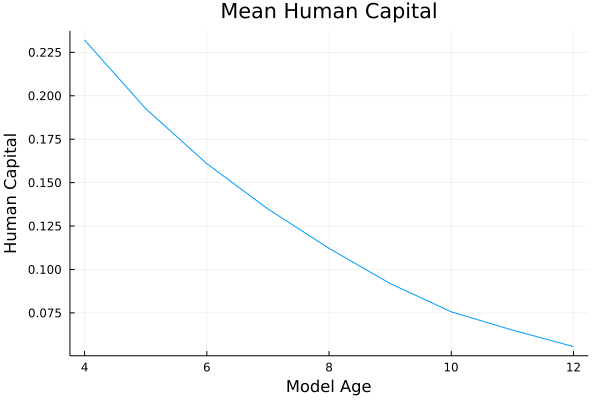
\includegraphics[scale =0.5]{mean_hc}
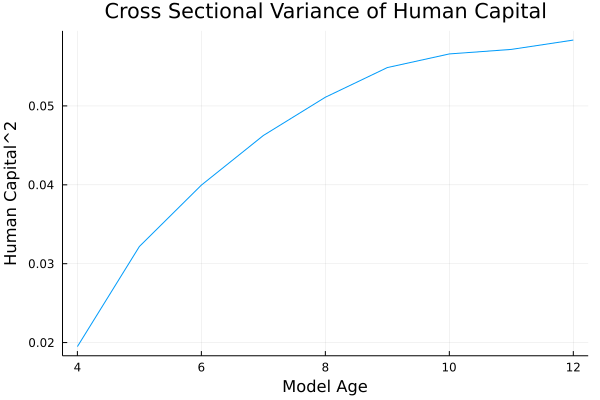
\includegraphics[scale =0.5]{var_hc}
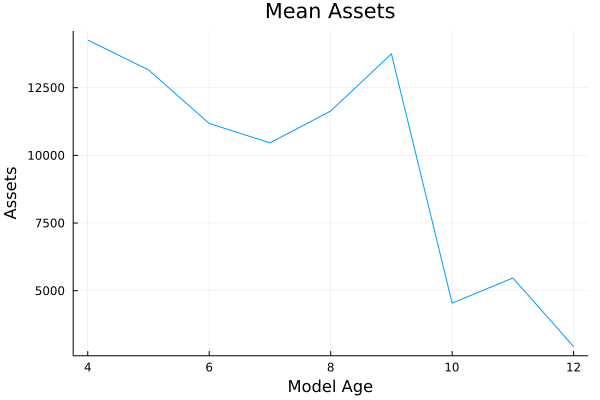
\includegraphics[scale =0.5]{mean_assets}
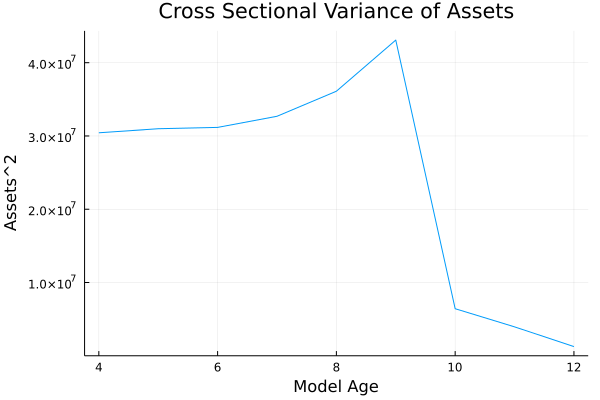
\includegraphics[scale =0.5]{var_assets}

\end{center}

We can see that average human capital starts relatively high and then decreases as agents experience more human capital shocks.  The cross-sectional variance of human capital steadily increases as agents experience the human capital shocks.  Average assets start relatively high and then dip as average earnings drop with human capital then increase again as agents save for the transfer to their children.  At $t=9$, assets drop substantially when parents make the transfer to their children.  The cross-sectional variance increases in $t=4, 5, 6, 7, 8$ as the human capital gets more disperse.  It then mechanically drops after parents make the transfer to their children.



\end{enumerate}

\end{document}

